\section{Accuracy of the model}
It is certainly important to investigate the accuracy of our model. 
However, performing an error analysis on a system with 1000 particles that strongly interact with each other is cumbersome. 
Therefore, we've only investigated our model on a two bodies system, which consists of a planet of 1 $M_{\oplus}$ rotating around the sun. 
With this approach, we hope to get an idea about the accuracy of our model.

\subsection{Elliptical orbit and conservation of energy}
One way to investigate the accuracy of the model is to check whether the calculations make sense physically. Due to Kepler's law, we expect the orbit of our planet around the sun should be elliptical. 
Also, since we are dealing with an isolated system, the total energy of the system, must be conserved. 
Therefore, it is meaningful to investigate whether our model satisfies these two properties.\\ 

\textbf{Remark}: In our case (with $\text{m}_{planet}=1\cdot M_{\oplus}$), the total energy of the system is \cite{Energy}
\[E_{tot}=\frac{1}{2}v_{planet}^2-\frac{GM}{r}+\frac{1}{2}Mv_{sun}^2-\frac{GM}{r}=\frac{1}{2}v_{planet}^2-2\frac{GM}{r}\]
With $M$ the mass of the sun, $r$ the distance between the planeet and the sun. 
Because the sun is at rest in our system, it's kinetic energy term drops out.\\

Since we chose to numerically integrate Newton's equation with a time step of $dt=1$ month, we expect that the calculations with planets which are close to the sun would be inaccurate. 
Because these planets have a much shorter orbital period than the earth. 
For example, Mercury has only a orbital period of 88 days. If we integrate with $dt=1$ month, we would only have roughly $4$ points for each turn around the sun, which is not very sufficient. 
Also, the stability of Leapfrog, when applied to an oscillatory system, is $\Delta t\leq 2/\omega$, with $\omega$ the angular frequency \cite{StabLeapfrog}. 
Because the x and y coordinates of our planets are in oscillatory motion, we would expect that for these planets that have a shorter orbital period(and thus larger $\omega$), the stability of Leapfrog is easily lost with large $\Delta t$.\\

Thus, we will first look at a planet that is 1$M_{\oplus}$, starting at a distance less than $1$ AU. 
After performing the integration with $dt=1$ over $10$ years, we obtained the following result:
\vspace{-20pt}
\begin{figure}[H]
\centering
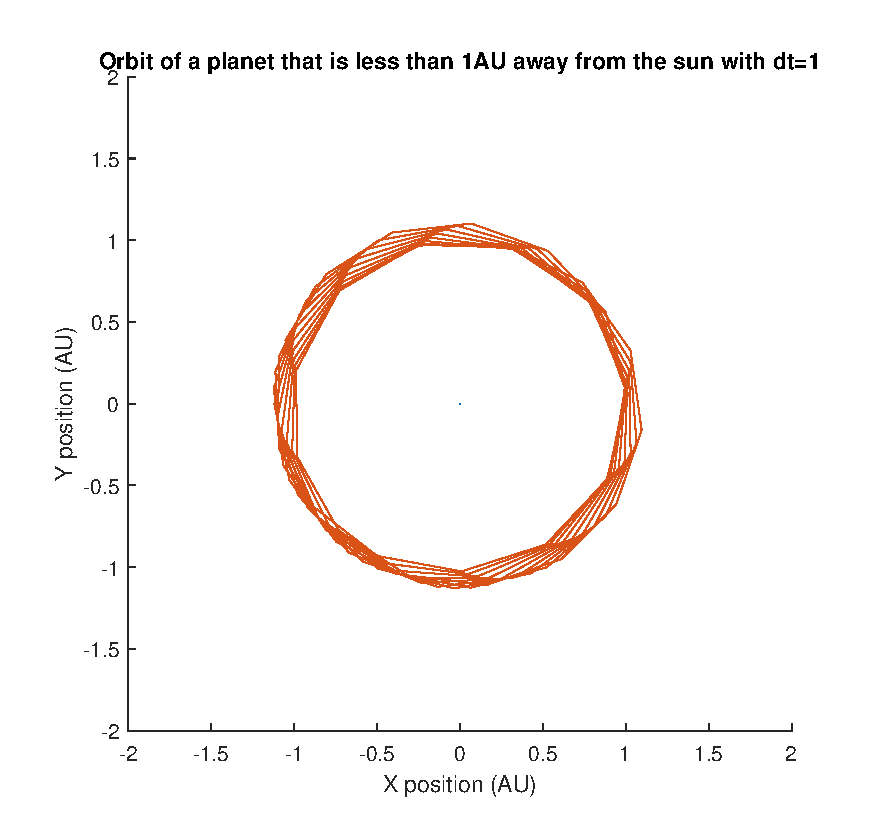
\includegraphics[width=0.6\textwidth]{Planeet_1AU_dt1_10jaar.eps}
\caption{Orbit of a planet of 1 $M_{\oplus}$ with a distance less than 1AU from the sun, integrated with $dt=1$ month over $10$ years.}
    \label{fig:Planet1AUdt1}
\end{figure}

As we can see from Figure \ref{fig:Planet1AUdt1}, the orbit is messy and not quite elliptical, which is expected. 
A calculation of the total energy also shows that the integration of the orbit is not accurate:\\

\begin{table}[htb]
\centering
\caption{The total energy of the system, which consists of a planet rotating less than 1AU away from the sun. The energy is calculated after each 20 time steps.}
\begin{tabular}{|l|l|l|l|l|l|l|l|}
\hline
k-th timestep&0&20&40&60&80&100&120\\ \hline
$E_{tot}$&-0.4080& -0.3539&   -0.3630&   -0.3643&   -0.3543&-0.3700&-0.4080\\ \hline
\end{tabular}
\label{tab:Planet1AUEnergy}
\end{table}

From Tabel \ref{tab:Planet1AUEnergy}, we see that the energy is not really conserved.\\

If we chose to integrate with $dt=0.5$ or $dt=0.25$, the accuracy of the orbit is greatly improved:

\begin{figure}[H]
	\centering
	\begin{subfigure}{0.45\textwidth}
	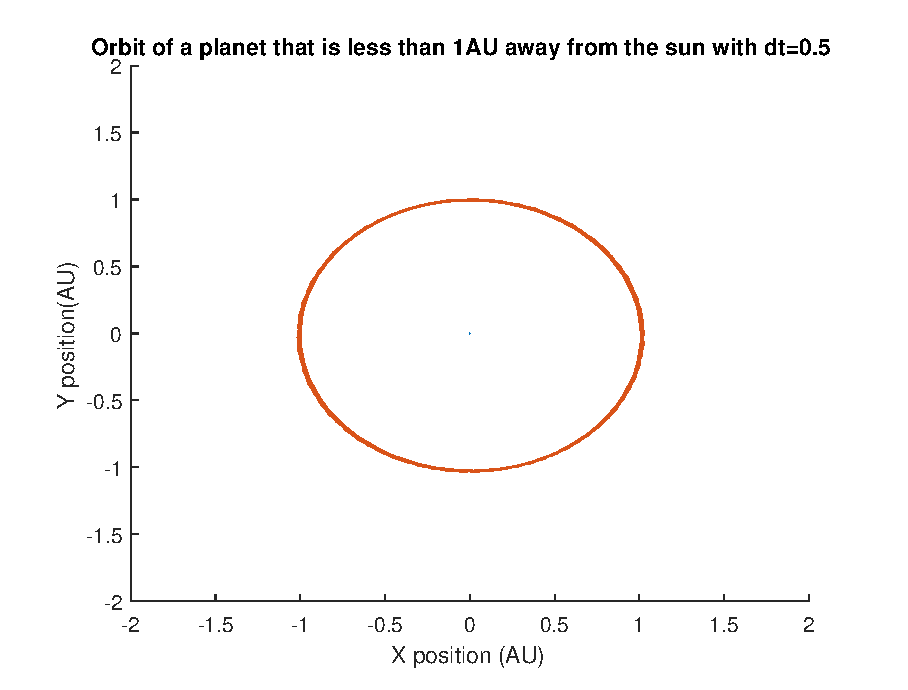
\includegraphics[width=\textwidth]{Planeet_1AU_dt05_10jaar.eps}
	\caption{Orbit calculation with $dt=0.5$}
	\end{subfigure}
	~
	\begin{subfigure}{0.45\textwidth}
	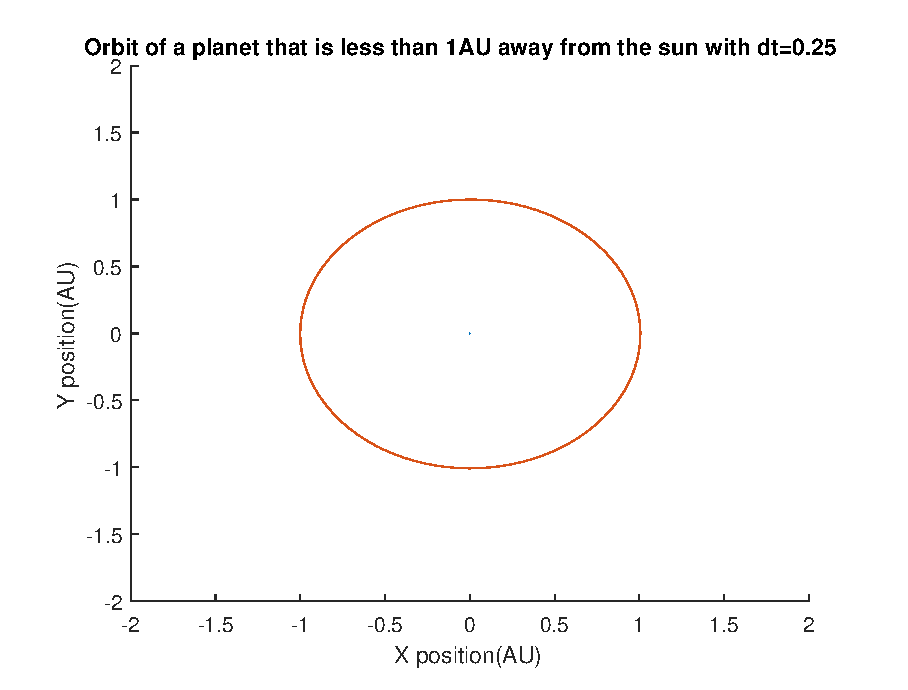
\includegraphics[width=\textwidth]{Planeet_1AU_dt025_10jaar.eps}
	\caption{Orbit calculation with $dt=0.25$}
	\end{subfigure}
	\caption{Orbit of a planet of 1 $M_{\oplus}$ with a distance less than 1 AU from the sun, integrated with $dt=0.5$ month and $dt=0.25$ month over $10$ years.}
\end{figure} 

But, when the planet is not too close to the sun, the integration with $dt=1$ is sufficient for a reasonable accuracy, which is shown in Figure \ref{fig:Planet2AUdt1}:

\begin{figure}[H]
\centering
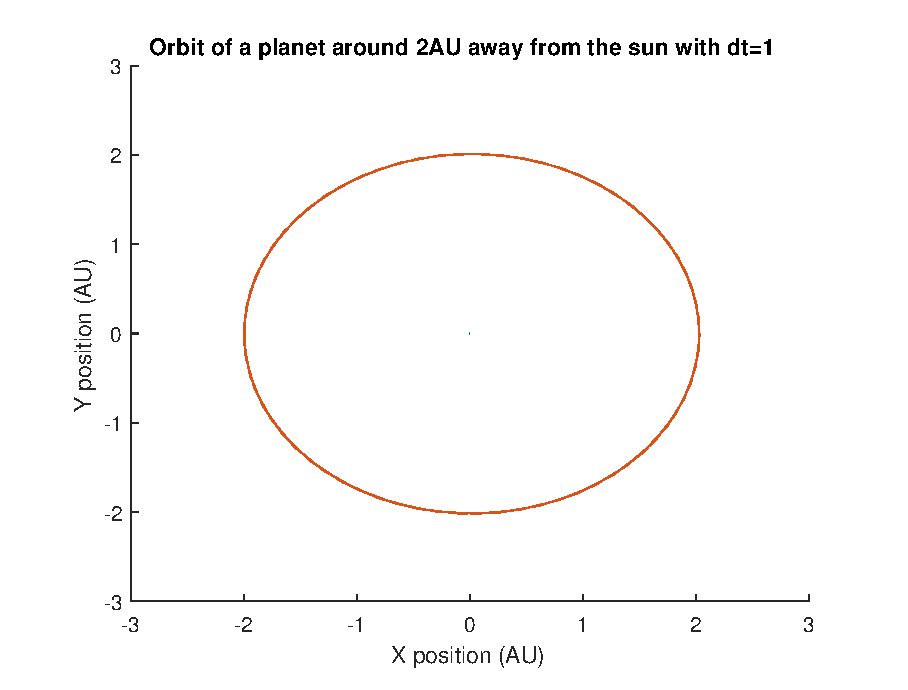
\includegraphics[width=0.6\textwidth]{Planeet_2AU_dt1_10jaar.eps}
\caption{Orbit of a planet of 1 $M_{\oplus}$ with a distance around 2AU from the sun, integrated with $dt=1$ month over $10$ years.}
    \label{fig:Planet2AUdt1}
\end{figure}

Also, the energy calculation (Table \ref{tab:Planet2AUEnergy}) shows that the energy is better conserved:

\begin{table}[htb]
\centering
\caption{The total energy of the system, which consists of a planet rotating around 2AU away from the sun. The energy is calculated after each 20 time steps.}
\begin{tabular}{|l|l|l|l|l|l|l|l|}
\hline
k-th timestep&0&20&40&60&80&100&120\\ \hline
$E_{tot}$&-0.2040&   -0.1996&   -0.2013&   -0.2005&   -0.2002&   -0.2015&   -0.2040\\ \hline
\end{tabular}

\label{tab:Planet2AUEnergy}
\end{table}

And if the planet is quite far from the sun, like around 5AU, then the energy is very well conserved and the orbit is also quite smooth:

\begin{figure}[H]
\centering
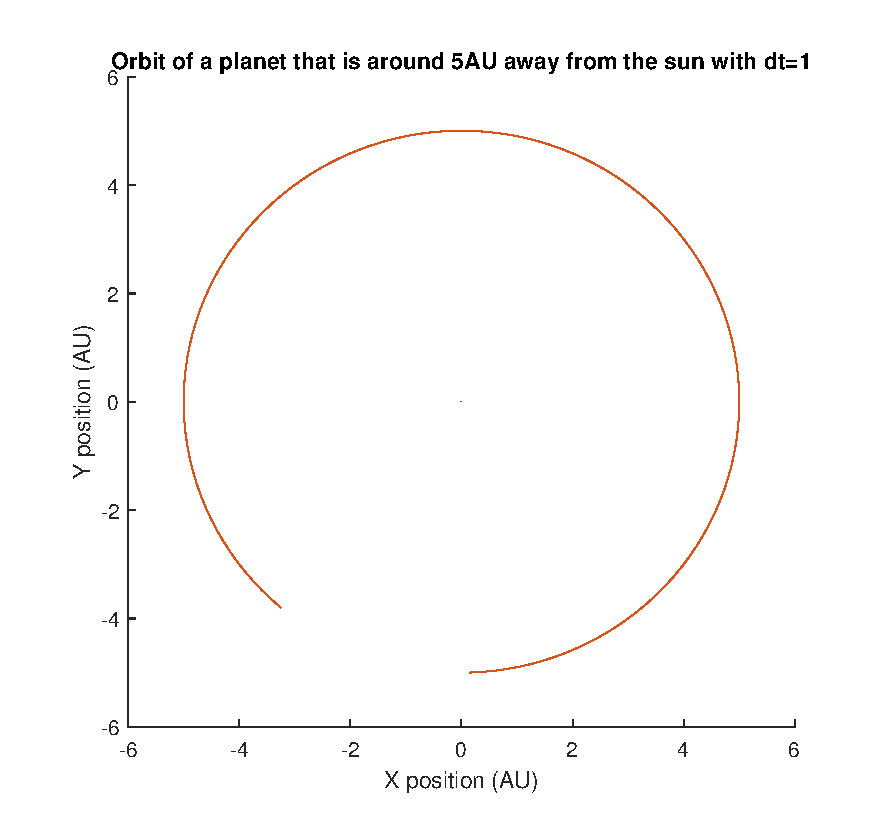
\includegraphics[width=0.6\textwidth]{Planeet_5AU_dt1_10jaar.eps}
\caption{Orbit of a planet of 1 $M_{\oplus}$ with a distance around 5AU from the sun, integrated with $dt=1$ month over $10$ years. Apparently, this planet has an orbital period longer than 10 years.}
    \label{fig:Planet5AUdt1}
\end{figure}

\begin{table}[htb]
\centering
\caption{The total energy of the system, which consists of a planet rotating around 5AU away from the sun. The energy is calculated after each 20 time steps.}
\begin{tabular}{|l|l|l|l|l|l|l|l|}
\hline
k-th timestep&0&20&40&60&80&100&120\\ \hline
$E_{tot}$&-0.0816&   -0.0815&   -0.0815&   -0.0815&   -0.0815&   -0.0815&   -0.0816\\ \hline
\end{tabular}
\label{tab:Planet5AUEnergy}
\end{table}

Since most of the bodies in our simulation is not too closed to the sun. 
The above results indicate that our model is not too inaccurate.

\subsection{Richardson Extrapolation}
Another more mathematical way to investigate the error of our integration is with Richardson Extrapolation. 
Let $Q(h)$ be the approximation using step size $h$. 
Then, the Richardson Extrapolation formula \cite{Richardson} gives an estimate for the order $p$ of the used numerical method:
\[\frac{Q(2h)-Q(4h)}{Q(h)-Q(2h)}=2^p\]

Therefore, we calculated the final position(thus after 10 years) of a planet which starts in a distance around 5AU from the sun, with $dt=1$, $dt=0.5$ and $dt=0.25$ and applied the Richardson Extrapolation formula. 
The result is shown in Table \ref{tab:Richardson5AU}:

\begin{table}[htb]
\centering
\caption{The final position of a planet that is around 5AU away from the sun, calculated with three different step size, namely $dt=1$, $dt=0.5$ and $dt=0.25$.}
\begin{tabular}{|l|l|l|l|}
\hline
dt (month)&1&0.5&0.25\\ \hline
x position (AU)&-3.2505&   -3.1469&   -3.0978\\ \hline
y position (AU)&   -3.8003&   -3.8859&   -3.9250\\ \hline
\end{tabular}
\label{tab:Richardson5AU}
\end{table}

For the order of the x position, denoted as $p_x$, the formula gives $p_x\approx 1.0782$.\\
For the order of the y position, denoted as $p_y$, the formula gives $p_y\approx 1.1304$.\\ 

This is very surprising result, because Leapfrog is known as a second order method. We do not know the reason yet.
\subsection{Comments about accuracy of our results}
So what does this analysis of two bodies says anything about our results with for example 1000 bodies? From the above observation, we saw that the integration is inaccurate for planets too close to the sun. Therefore, in our simulations with more bodies, we avoid this inaccuracy by conditioning the initial distance of each planets to the center of mass to be more than 1 AU, since we are integrating with $dt=1$. Of course, this comes with the price that our model is less realistic, since we are omitting planets that are less than 1 AU to the sun. Certainly, we could have chose a smaller $dt$ for planets close to the origin, but that would also require somewhat more programming work.\\

The elliptical orbit that we observed with only one planet implies that we are integrating correctly(there is still a error of order 1, but at least we obtained a reasonable solution). With more bodies, we will also have collisions, in which we used Euler Forwards to determine the condition for collisions. So we expect that in our results, the order of the error for the position of the bodies would still be 1.\\

We also expect that the total energy is conserved in our simulations with more bodies. Since Leapfrog is known as a sympletic integrator, which has energy conserving property \cite{Leapfrogsympletic}. 